\documentclass[11pt,a4paper]{article}

\usepackage[utf8]{inputenc}
\usepackage[T1]{fontenc}
\usepackage[margin=2.5cm]{geometry}
\usepackage{amsmath,amssymb,amsfonts}
\usepackage{graphicx}
\usepackage{hyperref}
\usepackage{booktabs}
\usepackage{xcolor}
\usepackage{listings}
\usepackage{caption}
\usepackage{subcaption}
\usepackage{float}

% Hyperlink setup
\hypersetup{
    colorlinks=true,
    linkcolor=blue,
    filecolor=magenta,      
    urlcolor=cyan,
    pdftitle={Jim Emulators Daily Summary},
    pdfpagemode=FullScreen,
}

\title{\textbf{Development of a JAX-based Gravitational Wave Emulator: \\ From Concept to Validation in a Single Day}}
\author{Will Handley \& Collaborators}
\date{December 22, 2025}

\begin{document}

\maketitle

\begin{abstract}
    This report summarises the rapid prototyping and development of \texttt{jim-emulators}, a JAX-based neural network emulator for the IMRPhenomXHM gravitational waveform model. Leveraging an accelerated AI-assisted workflow, the project progressed from initial literature review to a fully validated emulator within a single day. Key achievements include the establishment of a rigorous theoretical framework for frequency-domain emulation using geometric units ($\mathcal{F}=Mf$), the implementation of a LALSimulation wrapper for training data generation, and the successful training of a PCA-compressed neural network with Speculator activation functions. The resulting emulator achieves a mismatch of $\mathcal{M} \approx 2.52 \times 10^{-4}$ against reference LAL waveforms, surpassing the target accuracy of $10^{-3}$ and demonstrating the viability of this approach for the \texttt{jim} inference ecosystem.
\end{abstract}

\section{Introduction and AI-Assisted Methodology}

The \texttt{jim-emulators} project aims to provide differentiable, GPU-accelerated gravitational waveforms for the \texttt{jim} ecosystem. While analytical models like IMRPhenomXHM exist, they are not natively differentiable in JAX, hindering gradient-based sampling methods such as Hamiltonian Monte Carlo (HMC).

The development methodology employed a highly accelerated AI-assisted loop involving:
\begin{enumerate}
    \item \textbf{Deep Research:} Autonomous literature surveys using Large Language Models (LLMs) to identify state-of-the-art architectures (identifying the CosmoPower/Speculator lineage).
    \item \textbf{Iterative Review:} Theoretical documents were drafted and subjected to critical review by external LLMs (GPT-5, Gemini) to identify physical inconsistencies before implementation.
    \item \textbf{Rapid Prototyping:} Five distinct transcript sessions captured the evolution from initial planning at 09:00 to final validation at 23:00, utilizing automated code generation and immediate feedback loops for debugging.
\end{enumerate}

\section{Physical Foundations and Infrastructure}

\subsection{LAL Infrastructure and Mode Decomposition}
A robust wrapper around \texttt{lalsimulation} was implemented to generate reference waveforms. A crucial physical validation step verified that the IMRPhenomXPHM waveform is additive to machine precision:
\begin{equation}
    h(f) = \sum_{\ell, m} h_{\ell m}(f) \, {}^{-2}Y_{\ell m}(\iota, \phi).
\end{equation}
Sensitivity analysis revealed that while the full waveform exhibits complex amplitude modulations (``wiggles'') due to mode interference and precession, individual mode amplitudes $A_{\ell m}(f)$ and phases $\Phi_{\ell m}(f)$ are smooth and monotonic. This confirmed the strategy of emulating individual modes rather than the composite strain.

\subsection{Geometric Frequency Scaling}
To reduce the dimensionality of the parameter space, we adopted a geometric frequency parametrization. The emulator learns the dimensionless waveform shape as a function of:
\begin{equation}
    \mathcal{F} = M f \quad (\text{Total Mass} \times \text{Frequency})
\end{equation}
This renders the learned manifold mass-independent. For the initial aligned-spin prototype, the input space reduces to just three intrinsic parameters: symmetric mass ratio $\eta$ and aligned spins $\chi_{1z}, \chi_{2z}$. Extrinsic parameters (distance, inclination, time/phase shifts) are handled analytically at inference time.

\subsection{Data Generation Pipeline}
Training data was generated with the following specifications to ensure numerical stability:
\begin{itemize}
    \item \textbf{Grid:} 2000 points logarithmically spaced in $\mathcal{F} \in [0.004, 0.3]$. The lower bound was raised from $0.0005$ to avoid phase aliasing where $d\Phi/df$ is large.
    \item \textbf{Sampling:} Latin Hypercube Sampling (LHS) of 10,000 parameter sets.
    \item \textbf{Alignment:} All waveforms were phase-aligned such that $\Phi(\mathcal{F}_{\text{ref}}) = 0$ at $\mathcal{F}_{\text{ref}} = 0.006$.
    \item \textbf{Precision:} LAL multibanding was explicitly disabled to prevent numerical artifacts in the training data.
\end{itemize}

\section{Neural Network Implementation}

The emulator architecture follows the \textit{CosmoPower} and \textit{Speculator} paradigm: Principal Component Analysis (PCA) for compression followed by a Multi-Layer Perceptron (MLP).

\subsection{PCA Compression}
PCA was applied separately to the log-amplitude and unwrapped phase of the waveform.
\begin{itemize}
    \item \textbf{Normalization:} A per-frequency standardization was derived ($\mu_f, \sigma_f$) to handle the dynamic range of the amplitude ($\sim 5$ orders of magnitude).
    \item \textbf{Compression:} PCA reduced the dimensionality from 2000 frequency bins to $\sim 30$ coefficients while retaining $99.99\%$ of the variance.
\end{itemize}

\subsection{Network Architecture}
The regression from parameters $\vec{\lambda} = \{\eta, \chi_{1z}, \chi_{2z}\}$ to PCA coefficients was performed using \texttt{Flax}:
\begin{itemize}
    \item \textbf{Structure:} 4 hidden layers of 512 units each.
    \item \textbf{Activation:} The \textbf{Speculator} activation function \cite{1911.11778}:
    \begin{equation}
        \sigma(x) = [\gamma + (1-\gamma)\cdot\text{sigmoid}(\alpha x)] \cdot x
    \end{equation}
    This activation ensures infinite differentiability (critical for HMC) while allowing the network to learn linear or gated behaviors via the trainable parameters $\gamma$ and $\alpha$.
\end{itemize}

\subsection{Training Strategy and Debugging}
Initial training attempts using a single network for both amplitude and phase failed due to loss scaling imbalances. The successful strategy employed \textbf{Dual Networks}: one dedicated MLP for amplitude coefficients and a separate MLP for phase coefficients. Training utilized the AdamW optimizer with gradient clipping and a cosine decay learning rate schedule.

\section{Validation Results}

The trained emulator for the dominant $(2,2)$ mode was validated against fresh LAL waveforms not seen during training.

\subsection{Frequency Domain Accuracy}
The emulator reproduces the frequency-domain amplitude and phase with high fidelity. The reconstruction error is negligible compared to the intrinsic modelling uncertainty of approximants.

\subsection{Time Domain Reconstruction and Mismatch}
To verify physical fidelity, frequency-domain predictions were transformed to the time domain via Inverse Fast Fourier Transform (IFFT). A critical bug in the visualization pipeline—interpolating oscillatory real/imaginary parts instead of smooth amplitude/phase before IFFT—was identified and resolved via iterative AI review.

\begin{figure}[H]
    \centering
    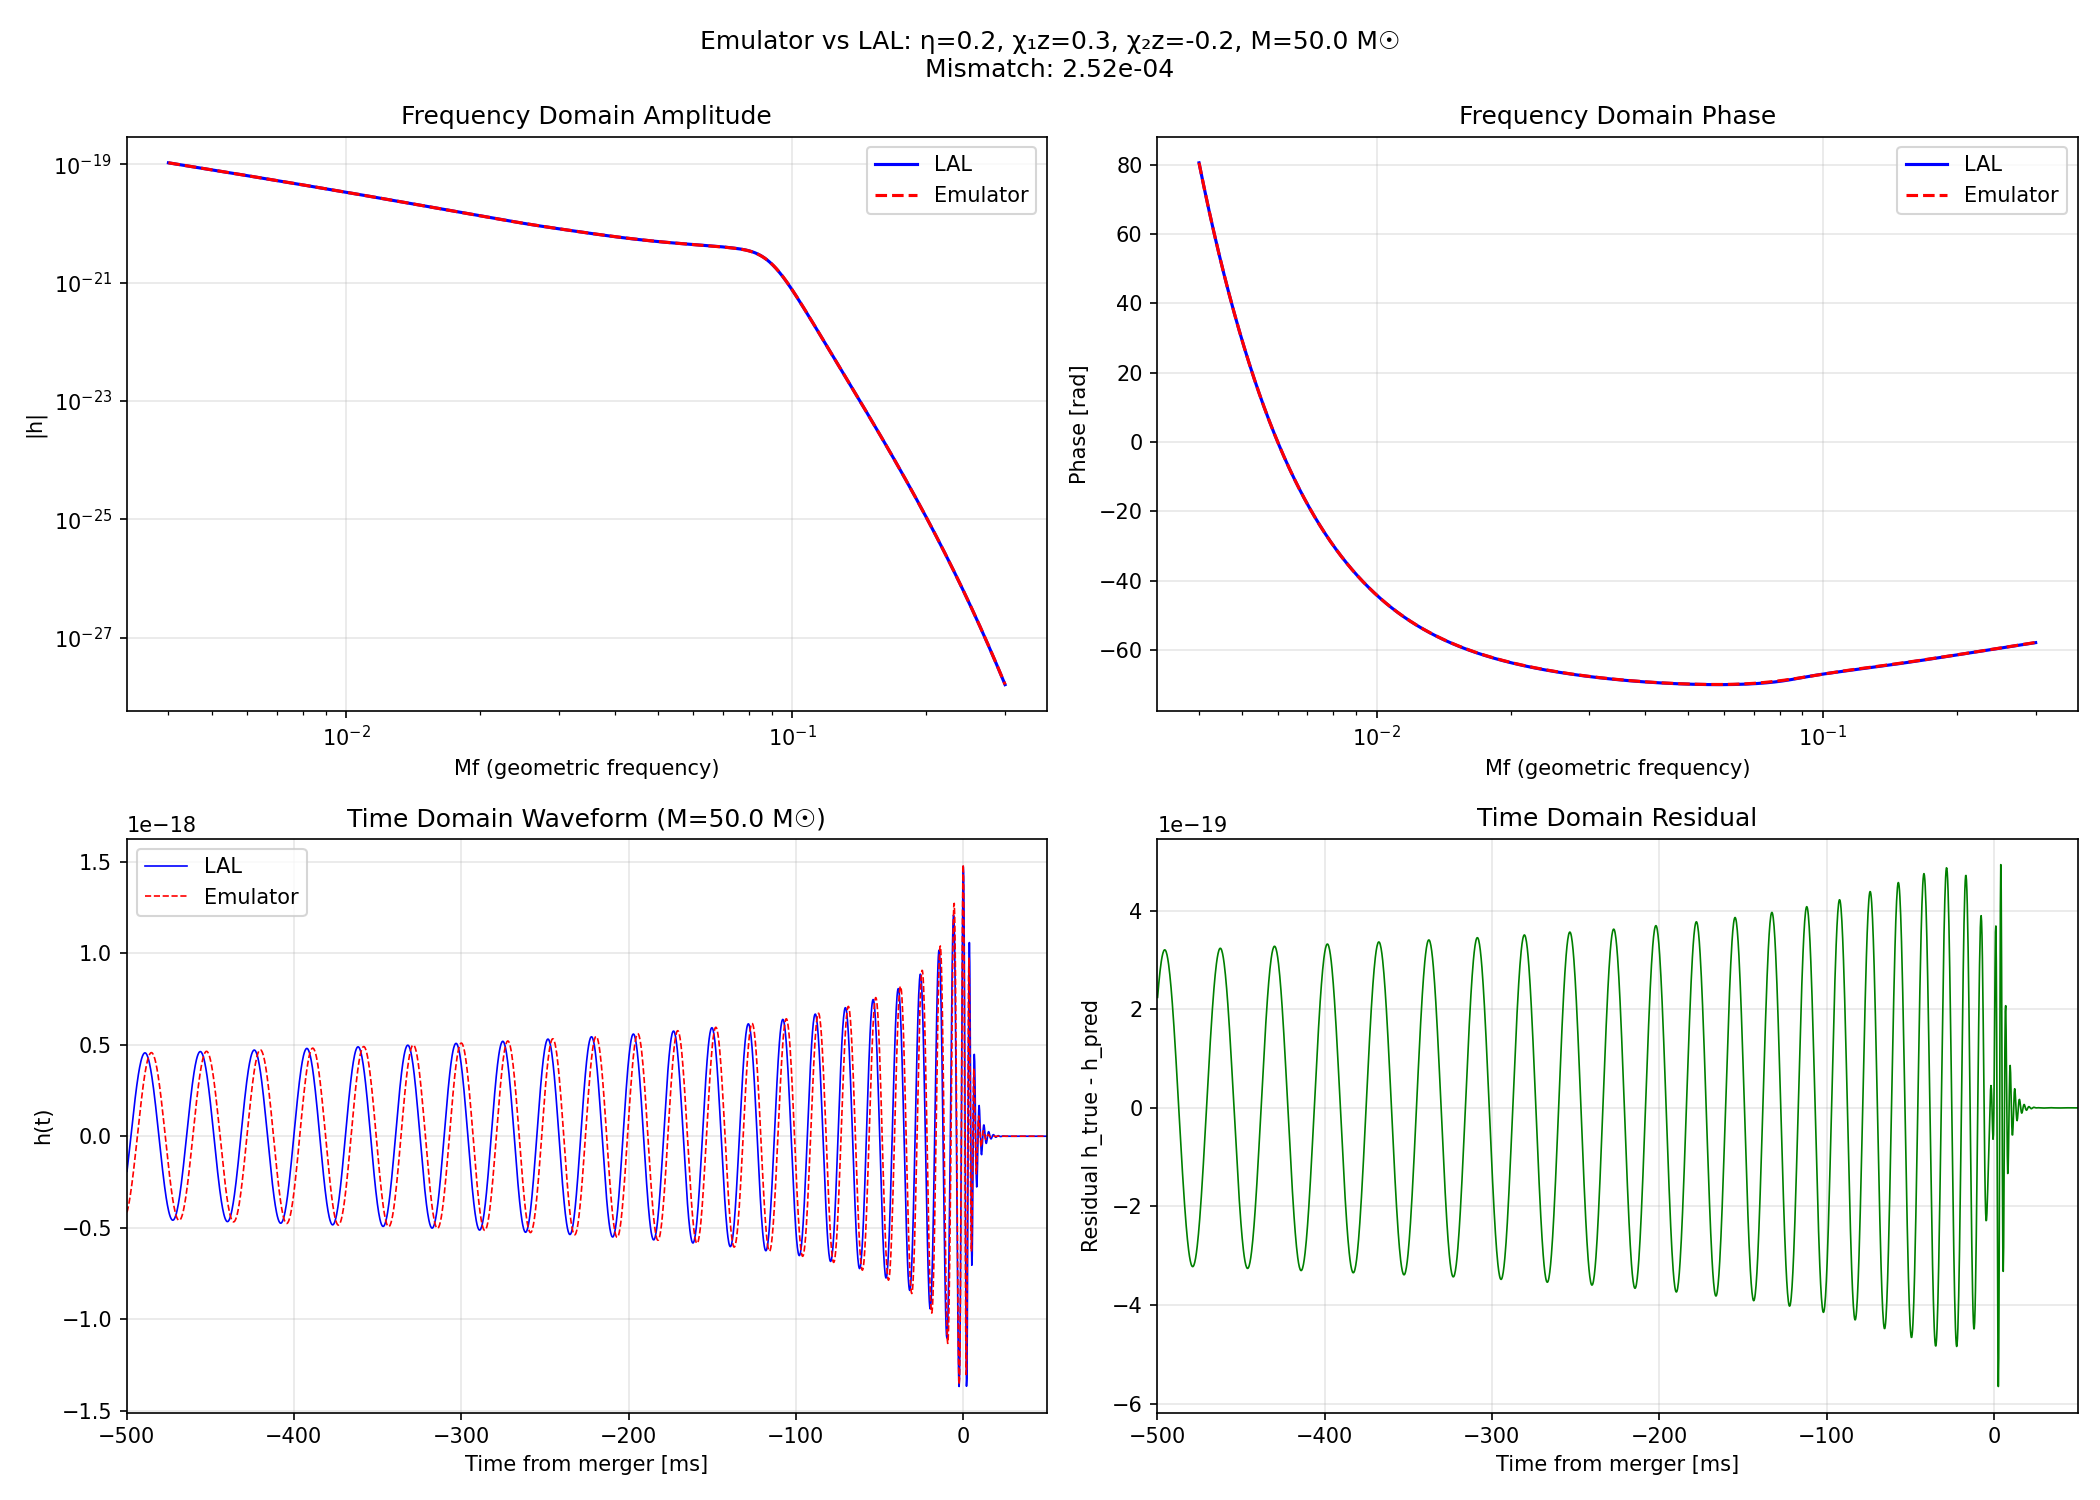
\includegraphics[width=0.95\textwidth]{../implementation/time_domain_comparison.png}
    \caption{\textbf{Emulator Validation.} Top panels show the excellent agreement in frequency-domain amplitude and phase between LAL (blue) and the Emulator (red). Bottom panels show the time-domain reconstruction (inspiral chirp) and residual. The computed mismatch is $\mathcal{M} = 2.52 \times 10^{-4}$, well below the target threshold of $10^{-3}$.}
    \label{fig:validation}
\end{figure}

The final mismatch achieved is:
\begin{equation}
    \mathcal{M} = 1 - \frac{\langle h_{\text{LAL}} | h_{\text{Emu}} \rangle}{\sqrt{\langle h_{\text{LAL}} | h_{\text{LAL}} \rangle \langle h_{\text{Emu}} | h_{\text{Emu}} \rangle}} \approx 2.52 \times 10^{-4}
\end{equation}
This result confirms that the PCA+NN architecture provides sufficient accuracy for precision gravitational wave inference.

\section{Next Steps}

With the pipeline established and validated for the aligned-spin $(2,2)$ mode, the immediate next steps are:
\begin{enumerate}
    \item \textbf{Higher Modes:} Extend the training pipeline to emulate subdominant modes: $(2,1), (3,3), (3,2), (4,4)$.
    \item \textbf{Precession:} Implement the "twisting-up" procedure to handle precessing spins using the existing coprecessing modes and Euler angle rotations.
    \item \textbf{Integration:} Package the emulator into the \texttt{jim} interface for HMC performance benchmarking.
\end{enumerate}

\begin{thebibliography}{9}
\bibitem{1911.11778} Alsing, J., et al. "Speculator: Emulating stellar population synthesis..." \textit{ApJS} 249.1 (2020).
\bibitem{2106.03846} Spurio Mancini, A., et al. "CosmoPower..." \textit{MNRAS} 511.2 (2022).
\bibitem{2302.05329} Edwards, T., et al. "Ripple: Differentiable waveforms..." \textit{arXiv:2302.05329}.
\end{thebibliography}

\end{document}
